\chapter{Manual práctico de HYDRA}
\label{ch:manual}

\section{Instalación}

El objetivo de este capítulo es proporcionar una ruta práctica para ejecutar los flujos principales con el menor número posible de decisiones ambiguas. El usuario puede trabajar de dos formas complementarias: instalando \pyhydra como librería Python, recomendado para desarrollo y uso desde scripts propios; o mediante la plataforma \hydra con Docker, recomendada para reproducir los notebooks, navegar la web y ejecutar los servicios sin configurar manualmente el entorno.

\begin{table}[htbp]
  \centering
  \caption{Formas recomendadas de uso de \pyhydra y \hydra.}
  \label{tab:manual_modos_uso}
  \begin{tabular}{p{0.28\textwidth}p{0.28\textwidth}p{0.32\textwidth}}
    \toprule
    Modo & Uso recomendado & Ventaja principal \\
    \midrule
    Instalación editable de \pyhydra & Desarrollo de módulos y uso desde scripts propios & Iteración rápida sobre el código fuente del núcleo \\
    \hydra + Docker + JupyterLab & Reproducir notebooks, revisar ejemplos completos y usar la web & Entorno cerrado con dependencias controladas \\
    \bottomrule
  \end{tabular}
\end{table}

Para instalación directa del núcleo \pyhydra en el entorno Python del usuario:

\begin{codeblock}
git clone https://github.com/navass11/pyhydra.git
cd pyhydra
pip install -e .
\end{codeblock}

La versión instalada puede comprobarse desde Python:

\begin{codeblock}
import pyhydra
print(pyhydra.__version__)
\end{codeblock}

\subsection{Despliegue del entorno Docker}

El entorno Docker pertenece al repositorio \hydra y es la vía recomendada cuando se quieren ejecutar los notebooks de ejemplo sin gestionar manualmente las dependencias. La imagen JupyterLab incluye \pyhydra con todas las dependencias extendidas ya instaladas (PyMC, NEOPRENE, HydroMT, hecdss, GeoPandas, etc.) y arranca JupyterLab en el puerto 8888. Para iniciar el entorno completo:

\begin{codeblock}
git clone https://github.com/navass11/HYDRA.git
cd HYDRA
docker compose -f docker/docker-compose.yml up -d
\end{codeblock}

Por defecto los datos se montan desde el subdirectorio \texttt{data/} del repositorio. Para apuntar a un directorio distinto (por ejemplo, un recurso compartido con proyectos de modelización ya existentes):

\begin{codeblock}
HYDRA_DATA_PATH="/ruta/a/datos" \
  docker compose -f docker/docker-compose.yml up -d
\end{codeblock}

El servicio \texttt{web} expone una interfaz de navegación de notebooks en el puerto 80. El acceso a JupyterLab se realiza en \texttt{http://localhost/jupyter/} y el backend de herramientas en \texttt{http://localhost/api/}.

\begin{figure}[p]
  \centering
  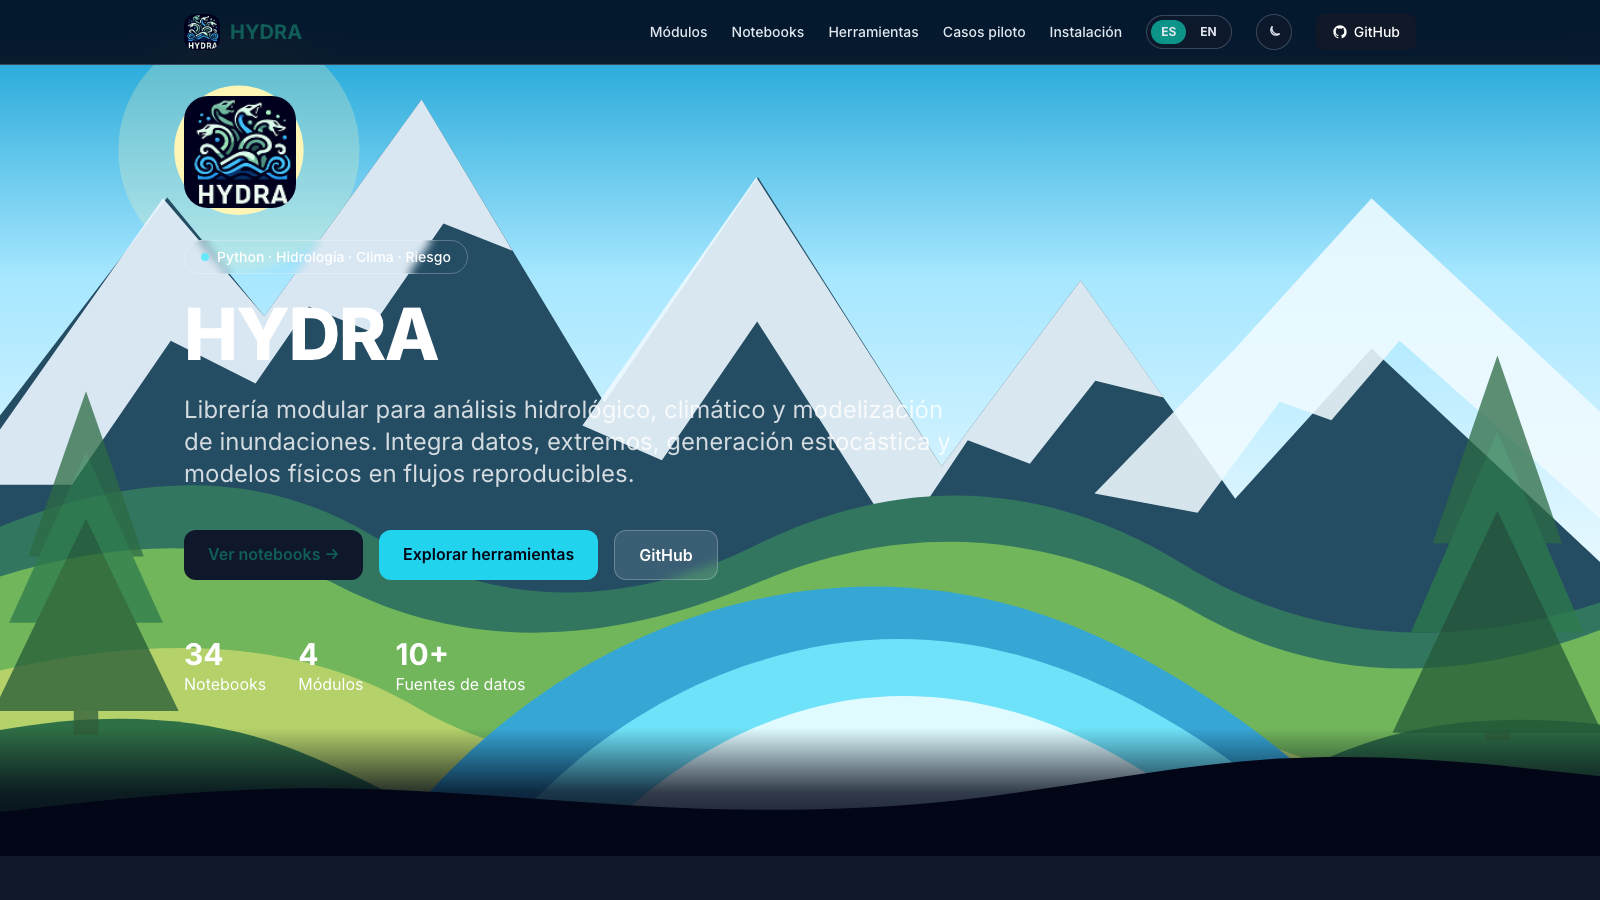
\includegraphics[width=0.96\textwidth]{figures/fig_hydra_web_home.png}
  \caption{Pantalla principal de la web de \hydra exportada desde el material de presentación de la tesis. La interfaz actúa como punto de entrada a los módulos, notebooks, herramientas, casos piloto e instalación, y traduce el núcleo \pyhydra a una experiencia navegable para usuarios técnicos.}
  \label{fig:hydra_web_home}
\end{figure}

\section{Criterios de uso como producto industrial}

\hydra se documenta en esta memoria como un \emph{framework} operativo ---no solo como un conjunto de scripts de investigación---. Por ello, cada flujo debe poder evaluarse con cuatro criterios: entrada trazable, transformación reproducible, salida estándar y registro suficiente para auditar el resultado. La \cref{tab:manual_contratos} resume estos contratos de uso.

\begin{table}[htbp]
  \centering
  \caption{Contratos operativos que debe cumplir un flujo reproducible con \hydra.}
  \label{tab:manual_contratos}
  \begin{tabular}{p{0.21\textwidth}p{0.25\textwidth}p{0.36\textwidth}}
    \toprule
    Elemento & Ejemplos & Requisito práctico \\
    \midrule
    Entradas & CSV, NetCDF, GeoTIFF, GeoJSON, DSS, ficheros HEC-RAS/HEC-HMS & Conservar fuente, fecha de descarga, versión del producto y sistema de referencia. \\
    Configuración & JSON/YAML, argumentos Python, parámetros de modelo & Separar parámetros del código y registrar umbrales, períodos, escenarios y semillas aleatorias. \\
    Salidas intermedias & Eventos, parámetros, hidrogramas, mapas simulados & Guardar productos que sean costosos de regenerar o necesarios para auditar decisiones. \\
    Salidas finales & Tablas, GeoTIFF, figuras, mapas de período de retorno & Exportar en formatos interoperables y acompañados de metadatos espaciales y temporales. \\
    \bottomrule
  \end{tabular}
\end{table}

La librería sigue una convención de datos sencilla: las series temporales se representan como \texttt{pandas.Series} o \texttt{pandas.DataFrame} con \texttt{DatetimeIndex}; los campos espaciales como \texttt{xarray.DataArray}, \texttt{xarray.Dataset} o raster GeoTIFF; y los modelos externos se tratan como proyectos versionables en disco. Esta decisión evita formatos propietarios dentro del núcleo de \pyhydra y facilita la integración con herramientas de consultoría, administración y visualización.

\section{Estructura del paquete}

\pyhydra se organiza en tres bloques principales que reflejan directamente la arquitectura descrita en el \cref{ch:arquitectura}:

\begin{itemize}
  \item \texttt{pyhydra.data\_sources} --- descarga, lectura y estandarización de fuentes de datos;
  \item \texttt{pyhydra.climate} --- análisis estadístico, generación estocástica, corrección de sesgo y downscaling;
  \item \texttt{pyhydra.modeling} --- automatización de modelos hidrológicos e hidráulicos.
\end{itemize}

Cada bloque expone sus funciones y clases principales directamente desde su \texttt{\_\_init\_\_.py}, de modo que el patrón de importación es siempre del tipo:

\begin{codeblock}
from pyhydra.climate.time_series import fit_gev, extract_block_maxima
from pyhydra.modeling.hydrology.hec_hms import HMSModel
from pyhydra.modeling.hydraulic.sfincs import setup_sfincs_model
\end{codeblock}

Los 26 notebooks generales de ejemplo catalogados por la web, excluyendo casos piloto y material interno de preparación de artículos, funcionan como guías ejecutables de las funcionalidades del paquete. La \cref{tab:notebooks} lista su correspondencia con los módulos. El catálogo fuente de la interfaz web contiene además 23 entradas de casos piloto, usadas para recorrer flujos completos de Besaya, M-30, Manning y Valencia desde el navegador.

\begin{figure}[htbp]
  \centering
  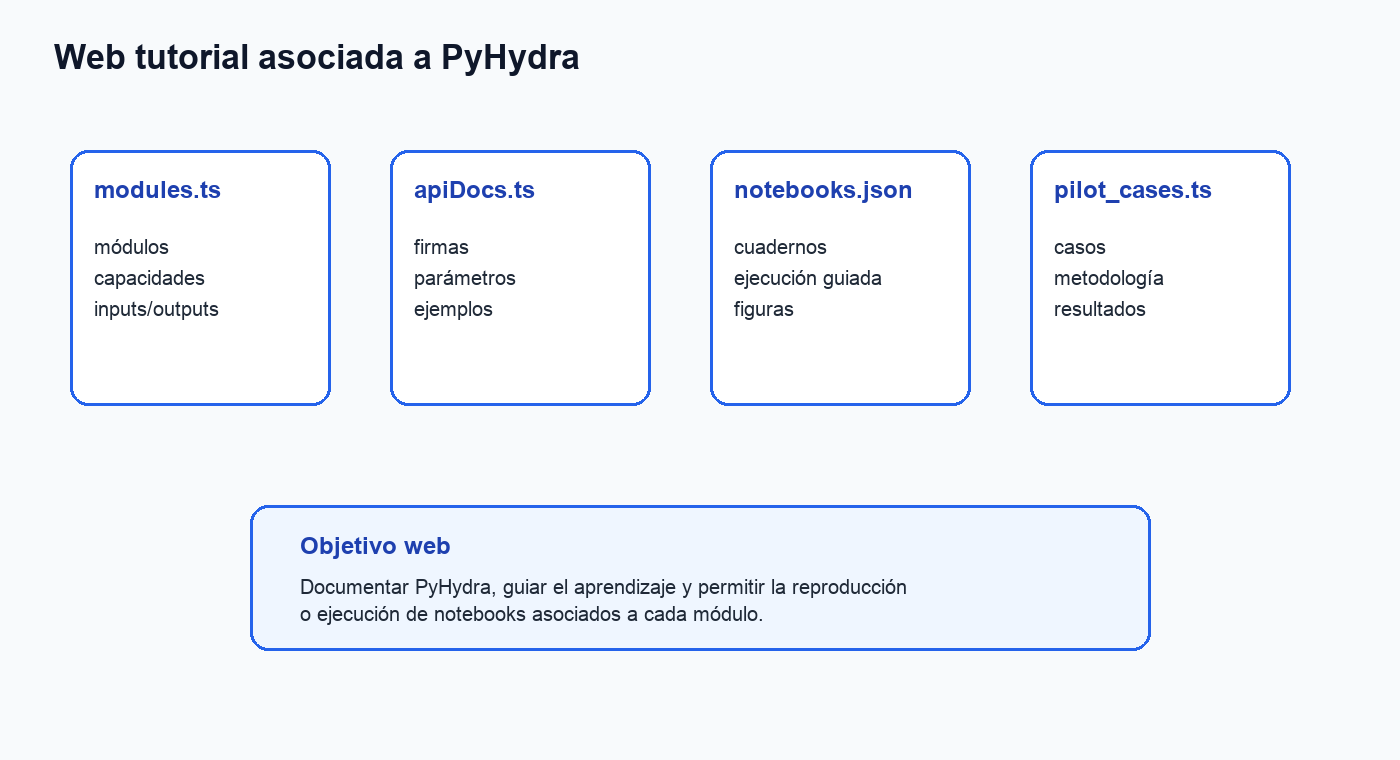
\includegraphics[width=0.94\textwidth]{figures/fig_hydra_web_tutorial.png}
  \caption{Estructura tutorial de la web asociada a \pyhydra. Los ficheros de catálogo conectan módulos, referencia de API, notebooks reproducibles y casos piloto, de modo que la documentación no queda separada del código ni de las evidencias computacionales usadas en la tesis.}
  \label{fig:hydra_web_tutorial}
\end{figure}

\begin{table}[htbp]
  \centering
  \caption{Responsabilidad técnica de cada bloque principal de \pyhydra.}
  \label{tab:manual_responsabilidades}
  \begin{tabular}{p{0.26\textwidth}p{0.31\textwidth}p{0.31\textwidth}}
    \toprule
    Bloque & Responsabilidad & Salida típica \\
    \midrule
    \texttt{data\_sources} & Obtener y normalizar datos externos sin alterar el dato bruto original. & NetCDF, CSV estandarizado, GeoTIFF, metadatos de descarga. \\
    \texttt{climate} & Transformar series y campos en eventos, distribuciones, escenarios sintéticos y productos estadísticos. & Tablas de eventos, parámetros, series sintéticas, mapas de retorno. \\
    \texttt{modeling} & Traducir datos internos de \hydra a los formatos de modelos físicos y recuperar resultados. & Proyectos HEC-HMS/HEC-RAS/SFINCS/SWAT, hidrogramas, rasters de calado. \\
    \bottomrule
  \end{tabular}
\end{table}

\small
\begin{longtable}{>{\raggedright\arraybackslash}p{0.55\textwidth}>{\raggedright\arraybackslash}p{0.33\textwidth}}
  \caption{Correspondencia entre notebooks y módulos de \pyhydra.}
  \label{tab:notebooks} \\
  \toprule
  Notebook & Módulo \pyhydra \\
  \midrule
  \endfirsthead
  \toprule
  Notebook & Módulo \pyhydra \\
  \midrule
  \endhead
  \path{data_sources/climate_change/CDS_download} & \path{data_sources.climate_change} \\
  \path{data_sources/climate_change/ESGF_download} & \path{data_sources.climate_change} \\
  \path{data_sources/rainfall/ERA5_download} & \path{data_sources.rainfall} \\
  \path{data_sources/rainfall/GPM_download} & \path{data_sources.rainfall} \\
  \path{data_sources/rainfall/PERSSIAN_download} & \path{data_sources.rainfall} \\
  \path{data_sources/rainfall/AEMET_download} & \path{data_sources.rainfall} \\
  \path{data_sources/rainfall/OGIMET_download} & \path{data_sources.rainfall} \\
  \path{data_sources/rainfall/Meteostat_download} & \path{data_sources.rainfall} \\
  \path{data_sources/river_discharge/GloFAS_download} & \path{data_sources.river_discharge} \\
  \path{data_sources/river_discharge/GRDC_download} & \path{data_sources.river_discharge} \\
  \path{data_sources/river_discharge/USGS_download} & \path{data_sources.river_discharge} \\
  \path{data_sources/soils/SoilGrids_download} & \path{data_sources.soils} \\
  \path{climate/event_extraction} & \path{climate.time_series} \\
  \path{climate/extreme_value_analysis} & \path{climate.time_series} \\
  \path{climate/spatial_analysis/regional_frequency_analysis} & \path{climate.spatial_analysis} \\
  \path{climate/spatial_analysis/bayes_hierarchical} & \path{climate.spatial_analysis} \\
  \path{climate/spatial_analysis/copulas} & \path{climate.spatial_analysis} \\
  \path{climate/spatial_analysis/compound_flooding} & \path{climate.spatial_analysis} \\
  \path{climate/spatial_analysis/interpolation} & \path{climate.spatial_analysis} \\
  \path{climate/stochastic_generation} & \path{climate.stochastic_generation} \\
  \path{climate/spatial_field_generation} & \path{climate.stochastic_generation} \\
  \path{climate/bias_correction} & \path{climate.bias_correction} \\
  \path{modeling/hydrology/HEC_HMS} & \path{modeling} \\
  \path{modeling/hydrology/SWAT} & \path{modeling} \\
  \path{modeling/hydraulic/SFINCS} & \path{modeling} \\
  \path{modeling/hydraulic/HEC_RAS} & \path{modeling} \\
  \bottomrule
\end{longtable}
\normalsize

\subsection{Notebooks como especificación ejecutable}

La documentación del producto no se apoya solo en la lectura del código fuente. Cada bloque de la librería se valida mediante notebooks que actúan como ejemplos reproducibles: contienen una descripción metodológica, datos sintéticos o de referencia, llamadas a la API y productos de salida. Esta estructura es especialmente importante en una tesis industrial, porque permite demostrar que \hydra no es un prototipo aislado, sino una herramienta con flujos de uso comprobables.

Además de los notebooks funcionales generales, el directorio del caso piloto de Los Corrales de Buelna, situado en \texttt{notebooks/pilot\_cases/}, documenta el origen de la línea metodológica. Este material complementa el capítulo de casos de estudio porque muestra el encadenamiento completo de la librería desde adquisición de datos hasta mapas de período de retorno.

\begin{table}[htbp]
  \centering
  \small
  \caption{Flujo del caso piloto de Los Corrales de Buelna documentado en notebooks.}
  \label{tab:manual_corrales_notebooks}
  \begin{tabular}{>{\raggedright\arraybackslash}p{0.34\textwidth}>{\raggedright\arraybackslash}p{0.25\textwidth}>{\raggedright\arraybackslash}p{0.29\textwidth}}
    \toprule
    Notebook & Módulos implicados & Función en el flujo \\
    \midrule
    \texttt{01\_data\_acquisition} & datos externos & Recopilación y organización inicial de series y cartografía. \\
    \texttt{02\_spatial\_interpolation} & \texttt{spatial\_analysis} & Reconstrucción espacial mediante IDW y kriging. \\
    \texttt{03\_extreme\_value\_analysis} & \path{time_series.extremes} & Ajuste GEV/GPD y curvas de período de retorno. \\
    \texttt{04\_design\_storm\_hms} & \texttt{modeling.hydrology} & Preparación de tormentas de diseño y entradas HEC-HMS. \\
    \texttt{05\_continuous\_simulation} & modelos externos & Simulación continua y gestión de hidrogramas. \\
    \shortstack[l]{\texttt{06\_hybrid\_event\_}\\\texttt{reconstruction}} & \texttt{hybrid\_downscaling} & Selección de eventos, MaxDiss y reconstrucción de hidrogramas. \\
    \texttt{07\_hec\_ras\_hydraulics} & \texttt{modeling.hydraulic} & Automatización de HEC-RAS para casos representativos. \\
    \texttt{08\_hybrid\_return\_periods} & \texttt{hybrid\_downscaling} & Reconstrucción de mapas y períodos de retorno por pixel. \\
    \bottomrule
  \end{tabular}
\end{table}

\subsection{Qué puede ejecutar un tercero}
\label{sec:reproducibilidad_tercero}

La reproducibilidad de \hydra se entiende en términos concretos: qué puede ejecutar un tercero mañana, con qué datos y en qué tiempo. La siguiente tabla clasifica los elementos reproducibles por tipo de dependencia y resultado esperado.

\begin{table}[htbp]
  \centering
  \small
  \caption{Elementos reproducibles de \hydra clasificados por disponibilidad, datos y tiempo estimado de ejecución.}
  \label{tab:reproducibilidad}
  \begin{tabular}{p{0.23\textwidth}p{0.09\textwidth}p{0.13\textwidth}p{0.13\textwidth}p{0.28\textwidth}}
    \toprule
    Elemento & Disp. & Datos & Tiempo & Resultado esperado \\
    \midrule
    Ajuste GEV sintético (MLE, L-mom., bayesiano) & Sí & Sintéticos & $<$5 min & Curvas de período de retorno con bandas de incertidumbre (fig.~5.1) \\[3pt]
    Análisis de inundación compuesta (cópulas) & Sí & Sintéticos & $<$5 min & Isolíneas AND/OR, MPDE (fig.~5.2) \\[3pt]
    Generación estocástica NEOPRENE (NSRP/STNSRP) & Sí & Sintéticos & $<$15 min & Series de lluvia sintéticas puntuales y multisitio \\[3pt]
    Corrección de sesgo delta/EQM & Sí & Sintéticos o ERA5, CMIP6 & $<$10 min & NetCDF corregido con señal de cambio preservada \\[3pt]
    Interpolación espacial y AFR & Sí & Sintéticos o AEMET & $<$10 min & GeoTIFF interpolado, cuantiles regionales \\[3pt]
    Descarga ERA5 (requiere cuenta CDS) & Sí & API abierta & Horas & NetCDF ERA5 horario/mensual \\[3pt]
    Descarga CMIP6 (requiere cuenta CDS) & Sí & API abierta & Horas & NetCDF de proyecciones por modelo y escenario \\[3pt]
    Simulación HEC-HMS (requiere HEC-HMS) & Sí & Modelos de referencia & 10--60 min & Hidrogramas DSS para 200 eventos sintéticos \\[3pt]
    Flujo hidráulico completo con SFINCS & Parcial & DEM + hidrogramas & Horas--días & Mapas de calado por evento, períodos de retorno por pixel \\[3pt]
    Caso piloto completo (Corrales de Buelna) & Parcial & Datos abiertos + modelo & Días & Distribución de calados, mapa de período de retorno \\
    \bottomrule
  \end{tabular}
\end{table}

Los elementos marcados como ``Parcial'' requieren adicionalmente un modelo calibrado o una licencia de software específica. Los primeros seis ítems pueden ejecutarse sin más requisito que tener instalado \pyhydra o el entorno Docker; son los más adecuados para una primera evaluación del marco.

\section{Referencia de la API}
\label{sec:manual_wiki_api}

La referencia completa de la API de \pyhydra ---incluyendo la firma de cada función, sus parámetros y el tipo de objeto devuelto--- se recoge en el \cref{app:api}. Las secciones siguientes ilustran el uso de cada bloque funcional mediante ejemplos representativos orientados a la aplicación práctica.

% ============================================================
\section{Bloque de datos (\texttt{pyhydra.data\_sources})}
% ============================================================

El bloque de datos agrupa cuatro módulos de acceso a fuentes externas con interfaces homogéneas: \texttt{rainfall} (ERA5, GPM, PERSIANN-CCS, AEMET, OGIMET), \texttt{river\_discharge} (GloFAS, GRDC, USGS), \texttt{climate\_change} (CMIP6 vía Copernicus CDS y ESGF) y \texttt{soils} (SoilGrids). Todos los módulos devuelven \texttt{pandas.DataFrame} o \texttt{xarray.Dataset} con metadatos de trazabilidad, y pueden ejecutarse desde los notebooks de ejemplo que documentan el proceso completo con datos reales para cada caso de estudio. La referencia de parámetros para cada función se recoge en el \cref{app:api}.

El criterio de diseño es minimizar la configuración manual: credenciales, dominios espaciales y períodos temporales se declaran explícitamente en el notebook de cada caso, de modo que la ejecución sea repetible sin intervención adicional. Cuando una fuente requiere registro (CDS, NASA Earthdata, ESGF, AEMET OpenData), los notebooks incluyen instrucciones paso a paso para obtener las credenciales necesarias.

El siguiente ejemplo ilustra la descarga de precipitación ERA5 y la lectura posterior del fichero resultante:

\begin{codeblock}
from pyhydra.data_sources.rainfall import download_era5
import xarray as xr

# Descarga precipitación horaria sobre la Península Ibérica (1979-2023)
download_era5(
    folder_out="data/era5/",
    api_key="UID:API_KEY",          # credenciales ~/.cdsapirc
    url="https://cds.climate.copernicus.eu/api",
    area=[44, -10, 35, 5],          # [N, W, S, E]
    variables_list=["total_precipitation"],
    years=range(1979, 2024),
)

# Lectura del NetCDF descargado como xarray.Dataset
ds = xr.open_mfdataset("data/era5/*.nc", combine="by_coords")
precip = ds["tp"] * 1000           # conversión m → mm
\end{codeblock}

Para descarga de caudales de una estación GRDC, el módulo devuelve directamente un \texttt{DataFrame} con índice de fechas:

\begin{codeblock}
from pyhydra.data_sources.river_discharge.grdc import read_grdc

# Lectura de fichero GRDC descargado del portal GRDC
Q = read_grdc("data/grdc/6335060_Q_Day.Cmd.txt")
# Q: pd.DataFrame con columnas ["date", "discharge"] (m3/s, NaN si falta/marcado)
\end{codeblock}

% ============================================================
\section{Bloque climático y estadístico}
% ============================================================

El bloque \path{pyhydra.climate} opera sobre las series y campos producidos por el bloque de datos. Se organiza en cinco submódulos con responsabilidades bien delimitadas:

\begin{description}
  \item[\texttt{time\_series}.] Detección de eventos (\texttt{extract\_events}) y análisis de extremos: ajuste GEV y GPD con cinco métodos de estimación (MLE, L-momentos, MAP, Fisher e MCMC), cálculo de niveles de retorno con incertidumbre y diagnóstico gráfico.

  \item[\texttt{spatial\_analysis}.] Interpolación espacial (kriging, IDW), análisis de frecuencia regional por el método de inundación índice, modelo GEV jerárquico bayesiano, cópulas gaussianas para eventos multivariantes (\texttt{FloodEventCopula}) y cópulas bivariantes con períodos de retorno conjuntos AND/OR y evento de diseño de máxima probabilidad para análisis de inundación compuesta (\texttt{BivariateCopula}).

  \item[\texttt{stochastic\_generation}.] Generación estocástica de precipitación con NEOPRENE, tanto puntual (\texttt{NSRPModel}) como multisitio (\texttt{STNSRPModel}), y generación de series hidro-climáticas generales con CoSMoS. Incluye además la generación de campos aleatorios espacialmente coherentes basados en variogramas.

  \item[\texttt{bias\_correction}.] Corrección de sesgo de proyecciones CMIP6: método delta (\texttt{delta\_method}) y mapeo cuantil (EQM, QDM, SDM) implementados en la clase \texttt{BiasCorrection}, con un único punto de entrada \texttt{BiasCorrection.fit\_transform} para las cuatro variantes.

  \item[\texttt{hybrid\_downscaling}.] Selección de eventos representativos por máxima disimilitud, reconstrucción de hidrogramas, interpolación de manchas de inundación y estimación del período de retorno por pixel. Las clases principales son \path{FloodEventSelector}, \path{HydrographReconstructor}, \path{FloodMapInterpolator} y \path{pixel_return_period}.
\end{description}

El flujo habitual combina los submódulos en secuencia: los extremos calibran los generadores estocásticos, la corrección de sesgo ajusta las proyecciones climáticas, y el downscaling híbrido convierte la serie sintética en mapas de impacto. Cada submódulo puede utilizarse de forma independiente cuando el caso de estudio no requiere la cadena completa. Los notebooks de ejemplo ilustran configuraciones representativas para cada bloque; la referencia de parámetros se recoge en el \cref{app:api}.

El siguiente ejemplo muestra el ajuste de una distribución GEV sobre máximos anuales, la estimación del nivel de retorno a T\,=\,100 años con intervalo de confianza bootstrap, y la representación gráfica del diagnóstico:

\begin{codeblock}
from pyhydra.climate.time_series import (
    extract_block_maxima, fit_gev, return_levels, return_level_ci,
    plot_return_levels,
)

# 1. Máximos anuales de precipitación diaria
ams = extract_block_maxima(precip_series, freq="YE")

# 2. Ajuste GEV por máxima verosimilitud
params = fit_gev(ams.values, method="mle")
# params: {"mu": ..., "sigma": ..., "xi": ...}

# 3. Niveles de retorno para T = [10, 25, 50, 100, 200, 500] años
rl = return_levels(params, T_values=[10, 25, 50, 100, 200, 500])

# 4. Intervalo de confianza al 90% por bootstrap (MLE + remuestreo)
point, lower, upper = return_level_ci(
    ams.values, T=100, method="mle",
    n_bootstrap=500, ci=0.90,
)

# 5. Figura de diagnóstico (QQ, PP y curva de retorno)
plot_return_levels(ams.values, params, T_range=(1.5, 500))
\end{codeblock}

Para la corrección de sesgo de proyecciones CMIP6 con el método delta sobre precipitación:

{\footnotesize
\begin{codeblock}
from pyhydra.climate.bias_correction import BiasCorrection

precip_corrected = BiasCorrection.fit_transform(
    obs=precip_obs_monthly,        # pd.Series observada (período histórico)
    hist=precip_cmip6_hist,        # pd.Series modelo histórico
    future=precip_cmip6_ssp585,    # pd.Series modelo futuro
    var="pr",                      # variable ("pr" o "tas")
    method="delta",                # "delta" | "eqm" | "qdm" | "sdm"
)
\end{codeblock}
}

% ============================================================
\section{Bloque de modelización (\texttt{pyhydra.modeling})}
% ============================================================

El bloque de modelización expone interfaces de automatización para cuatro motores de simulación externos organizados en dos familias:

\begin{description}
  \item[Hidrología.] \texttt{modeling.hydrology.hec\_hms} envuelve HEC-HMS con funciones de preparación de entradas meteorológicas, escritura en formato DSS, parametrización automática a partir de datos geoespaciales (curva número, tiempo de concentración, Muskingum) y lectura de resultados. \texttt{modeling.hydrology.swat} prepara ficheros de forzamiento para SWAT+ y lanza el ejecutable con control del período de simulación.

  \item[Hidráulica.] \texttt{modeling.hydraulic.sfincs} configura proyectos SFINCS desde geometría, DEM y series de caudal, calcula la condición de contorno aguas abajo con Manning y lanza el ejecutable. La lectura de resultados SFINCS en ensemble se realiza actualmente desde \texttt{modeling.hydraulic.sensitivity} mediante \texttt{load\_sfincs\_ensemble}, que extrae \texttt{hmax} de los ficheros \texttt{sfincs\_map.nc}. \texttt{modeling.hydraulic.hec\_ras} modifica ficheros de proyecto no estacionario e inserta hidrogramas de contorno sin salir de Python.
\end{description}

El patrón de uso es consistente en todos los módulos: preparar los datos en formatos internos de \pyhydra, llamar a las funciones de configuración, ejecutar el motor y leer los resultados mediante funciones de postprocesado. Los adaptadores aislan al usuario del formato propietario de cada motor, de modo que puede sustituirse un modelo hidráulico por otro sin modificar el código de análisis estadístico. Los notebooks de ejemplo documentan configuraciones completas para los casos del Besaya (HEC-HMS + SFINCS), Calle 30 (HEC-HMS + HEC-RAS) y SIMPCCe (SWAT); la referencia de parámetros se recoge en el \cref{app:api}.

El siguiente ejemplo ilustra la configuración y ejecución de SFINCS para un conjunto de hidrogramas representativos:

{\footnotesize
\begin{codeblock}
from pyhydra.modeling.hydraulic.sfincs import setup_sfincs_model, run_sfincs
from pyhydra.modeling.hydraulic.sensitivity import load_sfincs_ensemble

# 1. Crear proyecto SFINCS a partir de DEM e hidrograma de diseño
mod = setup_sfincs_model(
    basin_geom=basin_gdf,
    dem_path="data/dem/basin_5m.tif",
    output_dir="sfincs/event_0/",
    discharge_series=q_df,
    src_points=src_gdf,
    resolution=5.0,
    manning=0.04,
)
mod.write()

# 2. Ejecutar SFINCS
run_sfincs(
    model_dir="sfincs/event_0/",
    sfincs_exe="/opt/sfincs/sfincs",
)

# 3. Ejecución en bucle para todos los representativos
for i in range(200):
    mod = setup_sfincs_model(
        basin_geom=basin_gdf,
        dem_path="data/dem/basin_5m.tif",
        output_dir=f"sfincs/event_{i}/",
        discharge_series=hydrographs[i],
        src_points=src_gdf,
        resolution=5.0,
        manning=0.04,
    )
    mod.write()
    run_sfincs(
        model_dir=f"sfincs/event_{i}/",
        sfincs_exe="/opt/sfincs/sfincs",
    )

# 4. Lectura del ensemble SFINCS
ensemble = load_sfincs_ensemble(
    results_dir="sfincs/",
    subdir_pattern="event_{n}",
    nc_filename="sfincs_map.nc",
)
\end{codeblock}
}

% ============================================================
\section{Interfaz web de \hydra}
\label{sec:interfaz_web}
% ============================================================

Además de los notebooks de JupyterLab, \hydra incluye una interfaz web ligera que expone el catálogo de notebooks de forma navegable desde cualquier navegador, sin necesidad de acceder directamente al servidor de JupyterLab. La interfaz se sirve desde el contenedor \texttt{web} del entorno Docker y está construida con el \emph{framework} Astro compilado en estático, lo que la hace muy rápida. El catálogo canónico de la web se define en \path{web/src/data/notebooks.json}, con 49 entradas: 26 notebooks generales y 23 notebooks de casos piloto.

Las funcionalidades principales de la interfaz son:

\begin{itemize}
  \item Catálogo de notebooks generales y casos piloto, organizado por bloque funcional, con descripción de cada entrada y enlace directo al entorno JupyterLab para su ejecución.
  \item Visualización del estado del servidor JupyterLab (activo / inactivo) y resumen de kernels en ejecución, consultado al backend FastAPI.
  \item Acceso a la referencia de la API de \pyhydra organizada por módulo.
\end{itemize}

La interfaz web no sustituye a JupyterLab para la ejecución de código, sino que actúa como punto de entrada orientado a usuarios que necesitan explorar las capacidades de \hydra sin familiaridad previa con el entorno de notebooks. En un despliegue corporativo o en un entorno de proyecto compartido, esta interfaz es el primer punto de contacto para equipos técnicos no especializados en Python.

% ============================================================
\section{Flujo de trabajo completo}
\label{sec:flujo_completo}
% ============================================================

El flujo de trabajo típico de un estudio de inundación estocástica con \hydra encadena los módulos en seis etapas que corresponden a los pasos descritos en el \cref{ch:manual}:

\begin{enumerate}
  \item \textbf{Datos}: descargar precipitación (ERA5, AEMET), caudales (GRDC, GloFAS), suelos (SoilGrids) y proyecciones climáticas (CDS-CMIP6) para el dominio de estudio.
  \item \textbf{Eventos históricos}: extraer eventos independientes con \texttt{extract\_events} y ajustar distribuciones de extremos con \texttt{fit\_gev} o \texttt{fit\_gpd} para obtener los estadísticos de calibración de los generadores.
  \item \textbf{Generación estocástica}: calibrar y simular con \texttt{NSRPModel} (precipitación puntual), \texttt{STNSRPModel} (campo espacial) o \texttt{FloodEventCopula} (eventos multivariantes de caudal).
  \item \textbf{Escenarios climáticos}: corregir el sesgo de las proyecciones CMIP6 con \texttt{BiasCorrection} y combinar con los generadores estocásticos para obtener eventos bajo escenarios futuros.
  \item \textbf{Simulación}: seleccionar eventos representativos con \texttt{maxdiss}, ejecutar HEC-HMS o SWAT para obtener hidrogramas, y lanzar SFINCS o HEC-RAS para los mapas de calado.
  \item \textbf{Postprocesado}: reconstruir todos los mapas con \texttt{FloodMapInterpolator}, calcular períodos de retorno por pixel con \texttt{pixel\_return\_period} y exportar los productos finales con \texttt{save\_return\_period\_geotiffs}.
\end{enumerate}


La \cref{app:flujo_completo} recoge el esquema Python completo de este flujo, con las llamadas principales desde la descarga de datos hasta la generación de mapas de período de retorno.

\section{Control de calidad y entrega de resultados}

En una aplicación industrial, el resultado de \hydra no debe limitarse al mapa final. El entregable debe permitir reconstruir cómo se ha pasado del dato bruto a la decisión técnica. La \cref{tab:manual_qa} propone una lista mínima de comprobaciónes para proyectos de inundación, sequía o cambio climático.

\begin{table}[htbp]
  \centering
  \caption{Controles de calidad recomendados en flujos de trabajo con \hydra.}
  \label{tab:manual_qa}
  \begin{tabular}{p{0.20\textwidth}p{0.35\textwidth}p{0.33\textwidth}}
    \toprule
    Fase & Control & Evidencia que debe conservarse \\
    \midrule
    Datos & Huecos, unidades, huso horario, CRS, duplicados y cambios de versión del producto. & Informe de calidad, metadatos de descarga y serie o raster bruto. \\
    Eventos & Independencia, sensibilidad al umbral, duración mínima y coherencia física del evento. & Tabla de eventos, parámetros usados y figura diagnostica. \\
    Estadística & Ajuste de marginales, dependencia, incertidumbre y extrapolacion a períodos de retorno altos. & Parámetros, intervalos de confianza, gráficos QQ/PP y semilla aleatoria. \\
    Modelos & Balance de masa, condición de contorno, ejecuciones fallidas y estabilidad numérica. & Ficheros de proyecto, logs, lista de simulaciones válidas y descartadas. \\
    Mapas & NoData, alineacion espacial, resolución, unidades, plantilla GeoTIFF y consistencia entre escenarios. & GeoTIFF final, plantilla usada, resumen de calados y mapas de control. \\
    \bottomrule
  \end{tabular}
\end{table}

La entrega recomendada incluye siempre un fichero de configuración del estudio, un registro de ejecución y una carpeta de productos intermedios. Esta estructura permite repetir solo una parte del flujo cuando cambia una hipótesis, sin volver a descargar datos ni relanzar simulaciones hidráulicas costosas.

\section{Buenas prácticas}

Para mantener reproducibilidad se recomienda fijar las versiones de las dependencias principales, conservar los metadatos de descarga (escenario, modelo, fechas, versión de API), separar datos brutos de productos procesados y registrar los parámetros de cada simulación junto a sus resultados.

La estructura de directorios recomendada para un proyecto \hydra es:

\begin{codeblock}
proyecto/
  config/         # parámetros del estudio (JSON/YAML)
  data/
    raw/          # datos originales sin modificar
    processed/    # datos transformados, corregidos
  models/
    hms/          # proyecto HEC-HMS
    sfincs/       # mallas y configuración SFINCS
    hecras/       # proyecto HEC-RAS
  results/
    events/       # hidrogramas sintéticos
    flood_maps/   # mapas de calado simulados
    return_periods/ # mapas finales de períodos de retorno
  notebooks/      # análisis y visualización
\end{codeblock}

Esta convención ayuda a identificar rápidamente qué puede regenerarse y qué constituye información original o costosa de obtener, y facilita que otro usuario pueda reproducir el flujo partiendo de los datos brutos.
